\chapter{Resultados e Discussões} \label{ch:RD}


Neste capítulo são apresentados os resultados obtidos com o projeto da arquitetura dos módulos do sistema e o seu desenvolvimento, juntamente com a documentação, os diagramas de engenharia de \textit{software} e o protótipo composto pela interface de usuário e a parte lógica do sistema.


\section{Módulos do sistema} \label{subsec:modules}

\subsection{Módulo de captura dos dados} 

O módulo de captura dos dados têm seu funcionamento ilustrado na figura \ref{img:capturadados}. Como dito anteriormente, periodicamente este módulo obtém informações da estação meteorológica \textit{Vantage Vue™} e os armazena na base de dados por meio do módulo de gerenciamento de dados. Para cumprir sua função, o módulo foi dividido em três \textit{scripts} escritos em \textit{Javascript} e executados em \textit{Node.js}. 

\imagem{0.55}{capturadados}{Módulos de captura e gerenciamento dos dados}{O Autor}

O primeiro \textit{script}, Script Agendador (a), é responsável por executar, a cada intervalo pré-determinado de tempo, uma \textit{thread} composta pelo Script Cliente (b). O Script Driver é um programa que se conecta à estação meteorológica utilizando \textit{socket TCP}, envia um comando de \textit{LOOP} (ver anexo \ref{anex:anexo1}), recebe a resposta do comando contendo os dados e em seguida converte as unidades de medida. O Script Cliente possui o papel de criar uma instância do Script Driver (c), e após o recebimento dos dados, salvá-los na base de dados por intermédio de uma requisição HTTP para a API RESTful.

O agendador do Node.js, utilizado no Script Agendador para capturar os dados em determinados períodos de tempo, possui a mesma sintaxe do GNU crontab \cite{SITEGNUCRONTAB, SITEVIVALINUXCRONTAB, NODECRON} onde cada asterisco representa uma medida de tempo de acordo com o seguinte padrão:
 
\centerline{[minutos] [horas] [dias do mês] [mês] [dias da semana]}

\sourcecode{Configuração do intervalo de execução no Script Agendador}{cron}{javascript}{cron.js}

No exemplo do código acima o Script Cliente é executado por uma \textit{thread} a cada 15 (quinze) minutos.

\subsection{Módulo de gerenciamento dos dados}

O módulo de gerenciamento dos dados é formado pela API do sistema e pela base de dados. A API possui rotas relacionadas ao gerenciamento dos dados climáticos e dos dados dos usuários, como pode ser observado na subseção \ref{subsec:api}. Também foi construída utilizando-se da linguagem \textit{Javascript} e do ambiente de execução \textit{Node.js}, incluindo o modelo de documentos dos usuários e dos dados climáticos.
 
O servidor de banco de dados executa uma base não relacional baseada em documentos chamada MongoDB (ver subseções \ref{subsec:MongoDB} e \ref{subsec:datamodel}).

 \subsection{Módulo de exibição dos dados}

O módulo de exibição dos dados é constituído apenas da aplicação \textit{Ionic}, também escrita em \textit{Javascript}, porém com a adição de HTML e de CSS para construção das páginas. Neste caso, o \textit{Javascript} é empregado para dar funcionalidades às páginas renderizadas pelo HTML juntamente com CSS.

A aplicação Ionic pode ser compilada tanto para \textit{Web}, quanto para as principais plataformas móveis, devido a isso foi adotada tal tecnologia no projeto. O funcionamento da aplicação está detalhado na subseção \ref{subsec:interfaceComOUsurario}.


\section{Diagramas de Engenharia de Software} \label{sec:diagramas}
A etapa inicial no desenvolvimento de \textit{software} é compreender os relacionamentos entre o \textit{software} em projeto e o seu ambiente exterior. Esta etapa é essencial porque mostra como se dará a estrutura do sistema para se comunicar com o seu ambiente e quais serão os limites estabelecidos para o mesmo. A definição do sistema informa quais serão as funcionalidades implementadas e os recursos disponíveis \cite{sommerville2011engenharia}.

Os diagramas abordados serão o de caso de uso, de sequência e de atividade. Esses três diagramas proporcionam uma visão geral de cada etapa do funcionamento do sistema. Além disso, serão discutidos também os modelos de documentos referentes ao banco de dados adotado.

\subsection{Casos de uso} \label{subsec:casosDeUso}

As interações entre alguns elementos do sistema serão relatadas pelos diagramas de caso de uso seguintes, utilizando de uma abordagem abstrata e sem muitos detalhas de implementação, pois destinam-se apenas à oferecer uma compreensão do que o sistema faz, ou seja, define os requisitos funcionais do sistema \cite{sommerville2011engenharia}.

A figura \ref{img:caso_de_uso_1} mostra o caso de uso referente à utilização da aplicação cliente pelo usuário final, enquanto a figura \ref{img:caso_de_uso_2} demonstra as interações do sistema do ponto de vista da API.

\imagem{0.75}{caso_de_uso_1}{Diagrama de caso de uso referente ao usuário final}{O autor}
%\newpage

\begin{itemize}
	\item \textbf{Cadastrar usuário}

		\begin{itemize}
    		\item Atores
		    	\begin{itemize}
    		    	\item Usuário
		    	\end{itemize}

	    	\item Fluxo de eventos primário
			    \begin{enumerate}
	    		    \item o usuário deve se cadastrar informando seu nome, \textit{e-mail} e senha;
		        	\item a API armazena os dados do usuário;
		    	    \item o usuário é liberado para realizar o \textit{login}.
			    \end{enumerate}

    		\item Fluxo alternativo
			    \begin{itemize}
		    	   \item o usuário desiste de se cadastrar e cancela o caso de uso clicando no botão voltar.
	    		\end{itemize}

		\end{itemize}

	\item \textbf{Visualizar dados atuais}

		\begin{itemize}
		    \item Atores
	    		\begin{itemize}
		    	    \item Usuário
			    \end{itemize}
    
	    	\item Pré-condições
			    \begin{itemize}
		     	   \item o usuário deve estar autenticado
			    \end{itemize}

	    	\item Fluxo de eventos primário
			    \begin{enumerate}
		    	    \item o usuário deve efetuar o \textit{login} informando o \textit{e-mail} e a senha;
	    		    \item caso o usuário não seja autenticado, o sistema informa a respeito de credenciais inválidas e encerra o caso de uso;
		    	    \item a API autentica o usuário;
    			    \item o usuário é liberado para visualizar os dados atuais dos sensores da estação;
		        	\item após a visualização o usuário pode finalizar o caso de uso ou efetuar uma nova consulta se desejar.
			    \end{enumerate}

    		\item Fluxo alternativo
			    \begin{itemize}
    			   \item o usuário desiste de visualizar os dados atuais e cancela o caso de uso clicando no botão voltar.
			    \end{itemize}

		\end{itemize}

	\item \textbf{Visualizar histórico}

		\begin{itemize}
		    \item Atores
	    		\begin{itemize}
		    	    \item Usuário
	    		\end{itemize}

	    	\item Pré-condições
    			\begin{itemize}
			        \item o usuário deve estar autenticado
			    \end{itemize}

		    \item Fluxo de eventos primário
			    \begin{enumerate}
			        \item o usuário deve efetuar o \textit{login} informando o \textit{username} e a senha;
			        \item caso o usuário não seja autenticado, o sistema informa a respeito de credenciais inválidas e encerra o caso de uso;
			        \item a API autentica o usuário;
			        \item o usuário é liberado qual período cujo histórico será exibido;
			        \item o usuário seleciona as variáveis a serem exibidas no gráfico;
			        \item após a visualização do histórico o usuário pode finalizar o caso de uso se desejar.
			    \end{enumerate}

		    \item Fluxo alternativo
			    \begin{enumerate}
			        \item após a escolha do período de exibição do histórico o usuário pode voltar para a tela anterior e um novo período;
			        \item o histórico é exibido para o usuário;
			        \item após a visualização do histórico o usuário pode finalizar o caso de uso ou efetuar uma nova consulta se desejar.
			    \end{enumerate}

		    \item Fluxo alternativo
			    \begin{enumerate}
			        \item o usuário desiste de visualizar o histórico e cancela o caso de uso clicando no botão voltar.
			    \end{enumerate}
		\end{itemize}
\end{itemize}

\imagem{0.65}{caso_de_uso_2}{Diagrama de caso de uso do ponto de vista da API}{O Autor}
\newpage

\begin{itemize}


	\item \textbf{Salvar dados}

		\begin{itemize}
		    \item Atores
			    \begin{itemize}
			        \item API
			    \end{itemize}

		    \item Pré-condições
			    \begin{itemize}
			        \item o Módulo de captura dos dados realiza uma requisição HTTP solicitando o armazenamento dos dados
			    \end{itemize}

		    \item Fluxo principal
			    \begin{enumerate}
			        \item a API recebe a requisição;
			        \item a API requisita ao banco de dados a inserção dos dados;
        			\item a API responde a requisição HTTP informando o \textit{status} da operação (bem sucedida ou não).
			    \end{enumerate}
    
		    \item Fluxo alternativo
			    \begin{enumerate}
			        \item a API não consegue se conectar ao banco de dados, o caso de uso é cancelado.
			    \end{enumerate}
	
		    \item Pós-condições
			    \begin{itemize}
			       \item novas informações estão disponíveis no banco de dados para serem consultadas.
			    \end{itemize}
		\end{itemize}
		
		
	\item \textbf{Cadastrar usuário}

		\begin{itemize}
		    \item Atores
			    \begin{itemize}
			        \item API
			    \end{itemize}

		    \item Pré-condições
			    \begin{itemize}
			        \item a aplicação de usuário realiza uma requisição HTTP solicitando o armazenamento dos dados
			    \end{itemize}

		    \item Fluxo principal
			    \begin{enumerate}
			        \item a API recebe a requisição;
			        \item a API requisita ao banco de dados a inserção dos dados do usuário;
			        \item o banco de dados verifica a existência de algum registro contendo o mesmo \textit{e-mail}; 
        			\item a API responde a requisição HTTP informando o \textit{status} da operação (bem sucedida ou não).
			    \end{enumerate}
    
		    \item Fluxo alternativo
			    \begin{enumerate}
			        \item a API não consegue se conectar ao banco de dados, o caso de uso é cancelado.
			    \end{enumerate}
	
		    \item Pós-condições
			    \begin{itemize}
			       \item o usuário está apto a realizar seu \textit{login}.
			    \end{itemize}
		\end{itemize}

	\item \textbf{Autenticar usuário}

		\begin{itemize}
   			 \item Atores
			    \begin{itemize}
			        \item API
			    \end{itemize}

		    \item Pré-condições
			    \begin{itemize}
			        \item a aplicação de usuário realiza uma requisição HTTP solicitando a checagem das credenciais do usuário
			    \end{itemize}

		    \item Fluxo principal
			    \begin{enumerate}
			    	\item a API recebe a requisição;
			        \item a API requisita ao banco de dados a verificação dos dados;			
			        \item a API responde à requisição de \textit{login} enviando o \textit{token} de acesso do cliente.			     
			    \end{enumerate}

			\item Fluxo alternativo
			    \begin{enumerate}
			        \item a API não consegue se conectar ao banco de dados, então o caso de uso é encerrado.
			    \end{enumerate}
    
		    \item Fluxo alternativo
			    \begin{enumerate}
			        \item a API conecta-se ao banco de dados;
	        		\item a o banco de dados verifica que as credenciais do usuário são inválidas;
			        \item a API responde à requisição informando erro.
			    \end{enumerate}
		\end{itemize}
		
	\item \textbf{Servir dados entre datas}

		\begin{itemize}
    		\item Atores
			    \begin{itemize}
    	    		\item API
			    \end{itemize}

		    \item Pré-condições
			    \begin{itemize}
     		   		\item verificar qual o período dos dados requeridos pela aplicação cliente através dos parâmetros da requisição HTTP
			    \end{itemize}

			\item Fluxo principal
   	 			\begin{enumerate}
		     	   \item a API recebe a requisição;
			        \item a API requisita ao banco de dados os dados que foram obtidos no intervalo entre as datas;
		    	    \item a API envia os dados para a aplicação e encerra o caso de uso.
		   		 \end{enumerate}

			\item Fluxo alternativo
		    	\begin{enumerate}
			        \item a API não consegue se conectar ao banco de dados, então o caso de uso é encerrado.
		    	\end{enumerate}
    		
    		\item Fluxo alternativo
		    	\begin{enumerate}
			        \item não há dados referente ao período solicitado;
			        \item a API responde à requisição com um conjunto de dados vazio;
			        \item o caso de uso é encerrado.
		    	\end{enumerate}
		    	
		    \item Pós-condições
			    \begin{itemize}
        			\item o usuário pode visualizar as informações consultadas.
		    	\end{itemize}
		\end{itemize}
		
	\item \textbf{Servir o último registro}

		\begin{itemize}
    		\item Atores
			    \begin{itemize}
    	    		\item API
			    \end{itemize}

		    \item Pré-condições
			    \begin{itemize}
     		   		\item a aplicação de usuário realiza uma requisição HTTP solicitando os dados mais atuais
			    \end{itemize}

			\item Fluxo principal
   	 			\begin{enumerate}
		     	   \item a API recebe a requisição;
			        \item a API requisita ao banco de dados o registro mais recente;
		    	    \item a API envia os dados para a aplicação e encerra o caso de uso.
		   		 \end{enumerate}

			\item Fluxo alternativo
		    	\begin{enumerate}
			        \item a API não consegue se conectar ao banco de dados, então o caso de uso é encerrado.
		    	\end{enumerate}
    				    	
		    \item Pós-condições
			    \begin{itemize}
        			\item o usuário pode visualizar as informações consultadas.
		    	\end{itemize}
		\end{itemize}
\end{itemize}


\subsection{Diagrama de sequência} \label{subsec:diagSeq}

O diagrama de sequência apresenta a colaboração dinâmica entre as entidades do projeto. Diante dele é possível verificar as mensagens trocadas entre os objetos no decorrer do tempo \cite{SITESEQ}. A sequência de interações entre as entidades componentes do sistema no que tange a consulta de dados do histórico estão representadas pelo diagrama de sequência da figura \ref{img:sequencia2}.

\newpage

\imagem{0.63}{sequencia2}{Diagrama de sequência do sistema no contexto de visualização dos dados}{O Autor}


\begin{enumerate}
	\item O Usuário deseja ver o histórico das variáveis climáticas, então através da interface de usuário escolhe o período ao qual o histórico se refere;
	\item A aplicação solicita à API através de uma requisição HTTP contendo o momento de início e o momento do fim do período em seus parâmetros;     			\item A API recebe a solicitação e se comunica com a base de dados, então requere as informações quem possuem a data de leitura no intervalo escolhido;
	\item A base de dados retorna os dados em formato Json para a API;
	\item A API responde à requisição retornando os dados, também em formato Json, para a aplicação cliente;
	\item A aplicação cliente renderiza os gráficos utilizando o conjunto de dados obtidos.
\end{enumerate}

O diagrama de sequência para o caso de uso de visualização dos dados atuais possui a lógica de funcionamento idêntica ao diagrama da figura \ref{img:sequencia2}, diferenciando-se nos fatos de que o usuário não necessita preencher nenhum formulário, os métodos executados pela aplicação cliente e pela API são diferentes, e a aplicação não gera gráficos para este cenário, como pode ser observado na figura \ref{img:dados_atuais}. Os respectivos métodos utilizados pela aplicação cliente e pela API neste caso são mostrados abaixo.

\sourcecode{Método executado para a requisição dos dados atuais pela aplicação cliente}{metodo1}{javascript}{metodo1.js}

\sourcecode{Método executado pela API para a busca dos dados atuais}{metodo2}{javascript}{metodo2.js}

A figura \ref{img:sequencia3} demonstra o caso de obtenção dos dados da estação por parte do sistema, onde a API recupera dos dados provenientes da estação e os insere no banco de dados para futuras consultas.


\imagem{0.55}{sequencia3}{Diagrama de sequência do sistema no contexto de obtenção de dados}{O Autor}

\begin{enumerate}
	\item O Script Cliente inicia uma nova instância do Script Driver;
	\item O Script Driver envia através de uma conexão TCP o comando de LOOP para o \textit{datalogger} da estação;
	\item O \textit{datalogger} responde ao comando de LOOP retornando um pacote de 99 \textit{bytes} contendo os dados da última leitura da estação;
	\item O Script Driver retorna para o Script Client um Json contendo os dados já convertidos para as unidades mais usuais;
	\item O Script Cliente envia para a API, através de uma requisição HTTP, os dados coletados;
	\item A API solicita à base de dados a inserção das informações;
	\item A base de dados confirma a inserção das informações para a API;
	\item A API confirma para o Script Cliente o sucesso da operação.
\end{enumerate}

\subsection{Diagrama de atividades} \label{subsec:diagAtiv}

Os diagramas de atividade são semelhantes a fluxogramas, porque englobam a direção das informações entre as ações em uma atividade. Os estados no diagrama de atividades mudam para uma próxima etapa quando uma ação é executada \cite{SITEDIAGATIV}.  O diagrama de atividades da figura \ref{img:atividades1} ilustra o fluxo de controle de todo o sistema de consulta, desde a observação dos dados atuais, até a visualização do histórico das variáveis meteorológicas.

\imagem{0.64}{atividades1}{Diagrama de atividades do sistema}{O Autor}

\newpage

\subsection{Interface com o usuário} \label{subsec:interfaceComOUsurario}

A aplicação cliente ou interface de usuário contém sete telas, sendo: tela de início, tela de \textit{login}, tela de cadastro, tela de dados atuais, tela de seleção de período, tela de histórico e tela de sobre  (ver figura \ref{img:telas}). A tela inicial a ser exibida assim que o usuário é autenticado é a tela de dados atuais, a partir de então o usuário possui a liberdade de permanecer na mesma, consultar o histórico informando os dados necessários para tal ou efetuar o \textit{logoff}.

\begin{figure}[!htb]
\centering
    \caption{\label{img:telas} Telas da aplicação cliente}
    \subcaptionbox{\label{img:inicial} Abertura}{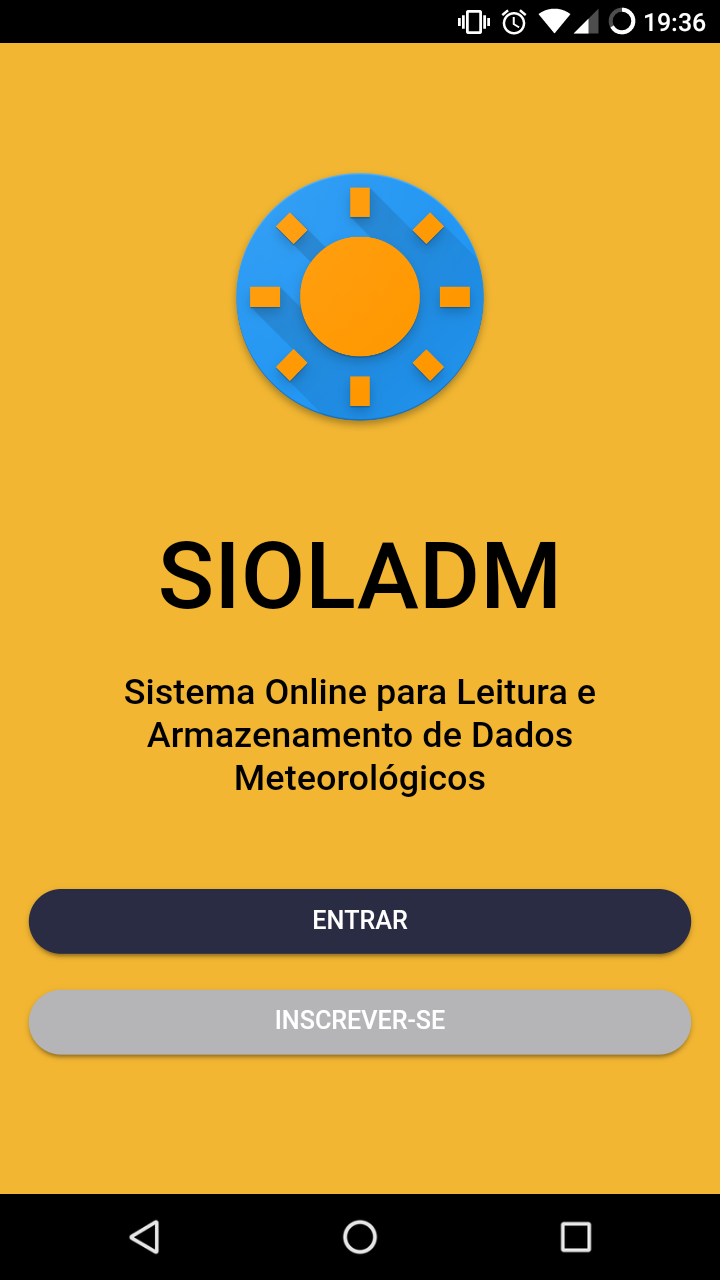
\includegraphics[scale=.12]{img/APP/inicial}}\qquad
    \subcaptionbox{\label{img:login} \textit{Login}}{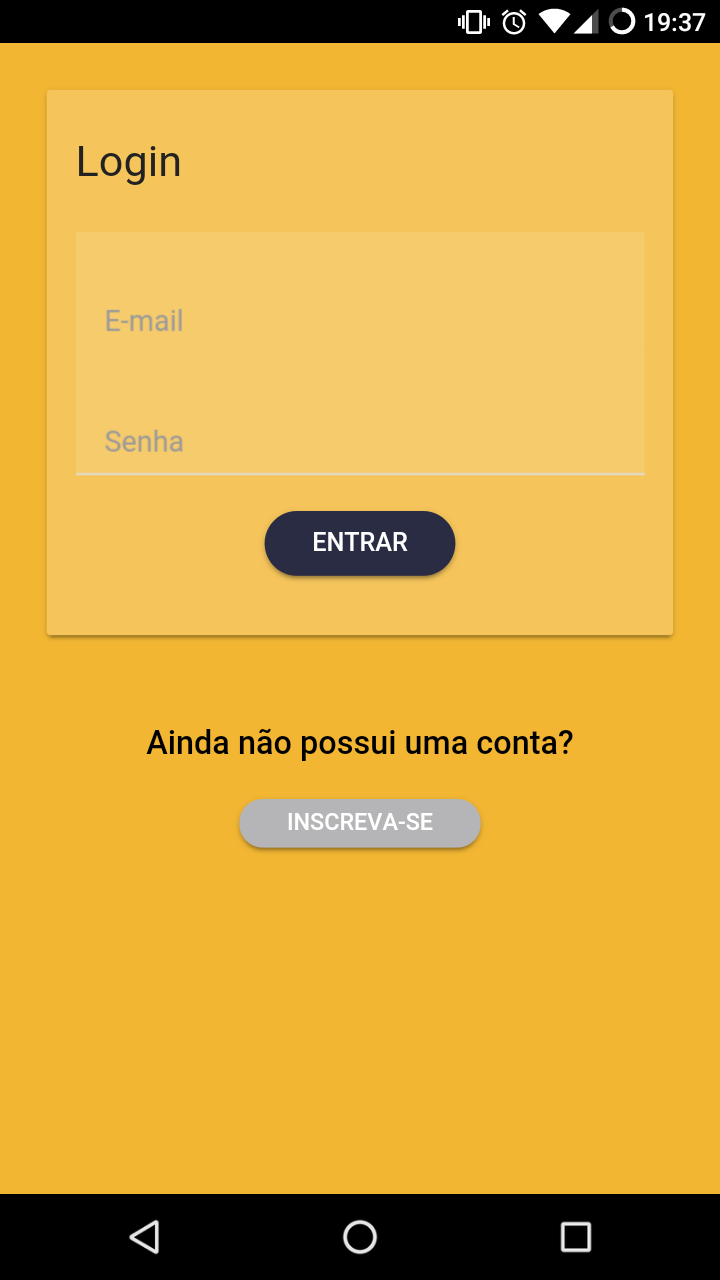
\includegraphics[scale=.12]{img/APP/login}}\qquad
    \subcaptionbox{\label{img:cadastro} Cadastro}{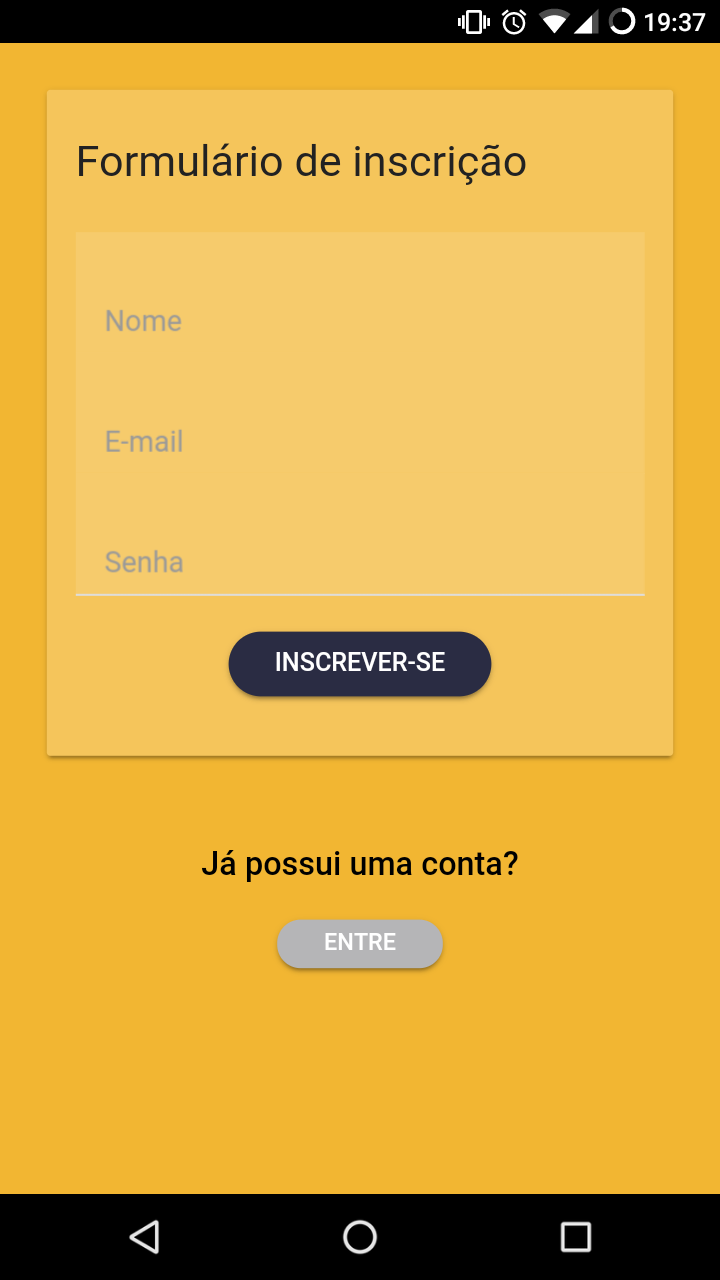
\includegraphics[scale=.12]{img/APP/cadastro}}\qquad
    \subcaptionbox{\label{img:hist-rel}Sobre}{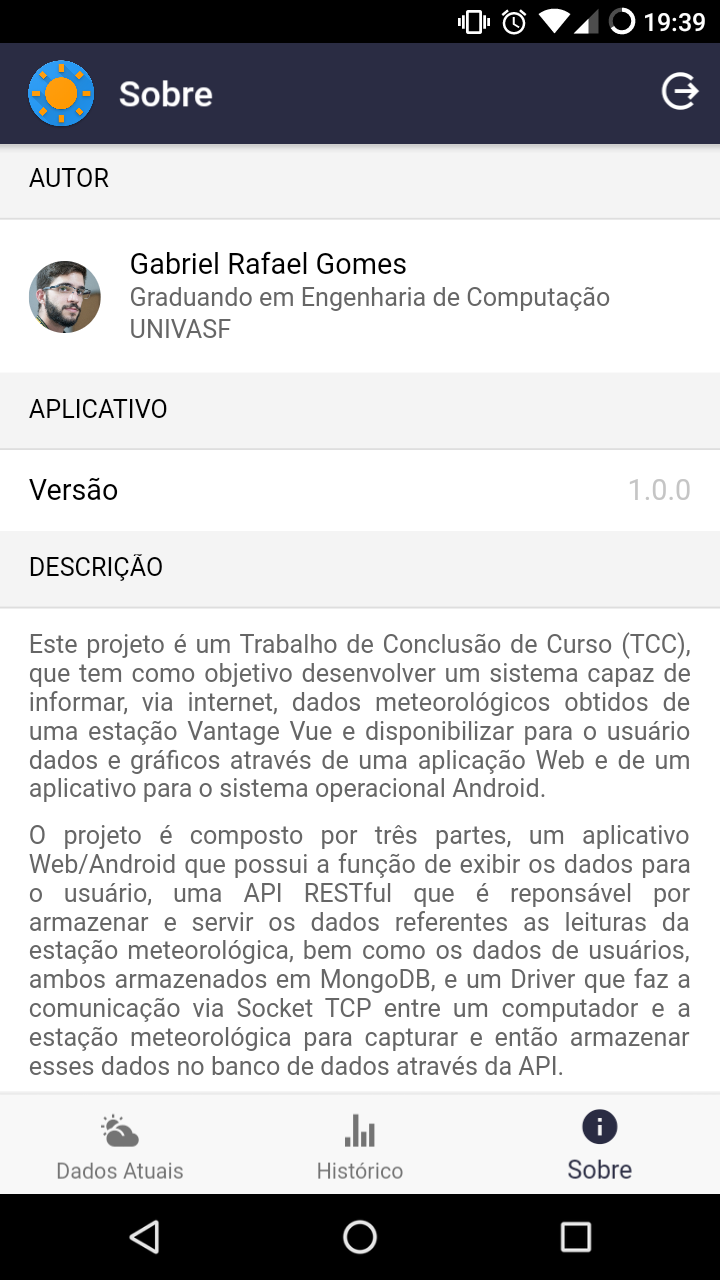
\includegraphics[scale=.12]{img/APP/sobre}}\\
    \vspace{1.5em}
    \subcaptionbox{\label{img:dados_atuais}Dados atuais}{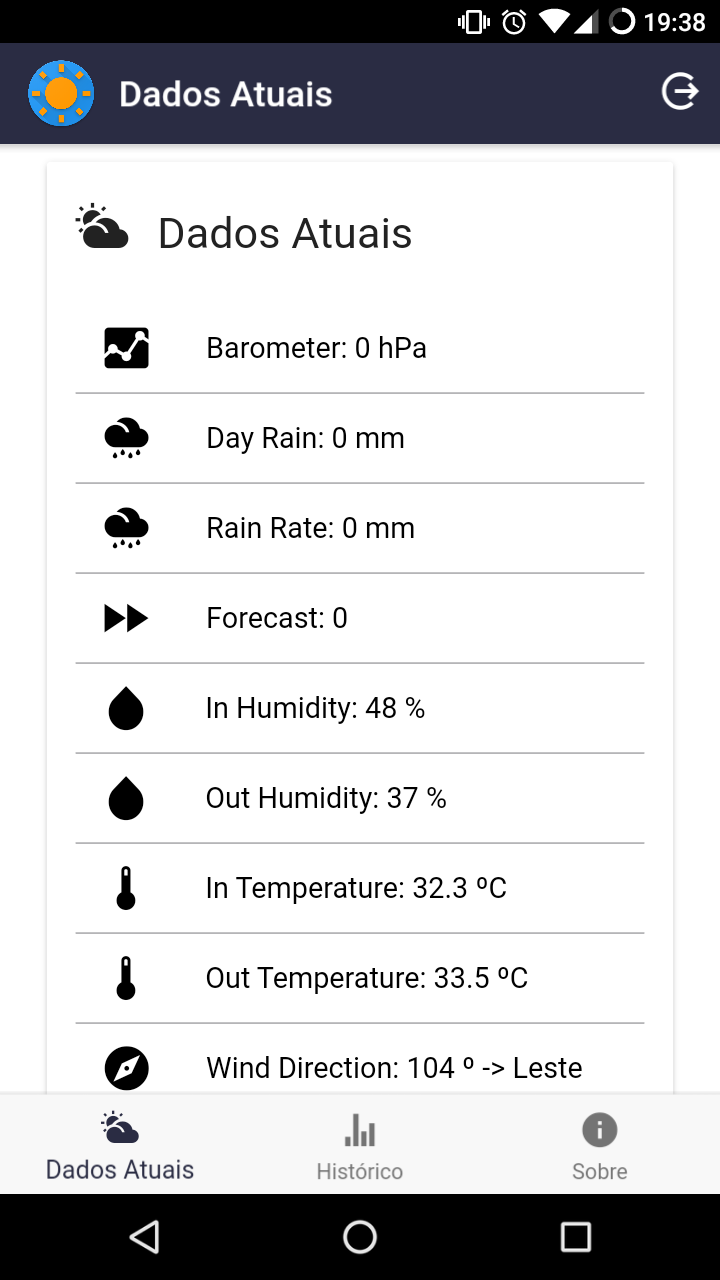
\includegraphics[scale=.15]{img/APP/atual}}\qquad
    \subcaptionbox{\label{img:hist-time}Seleção de período}{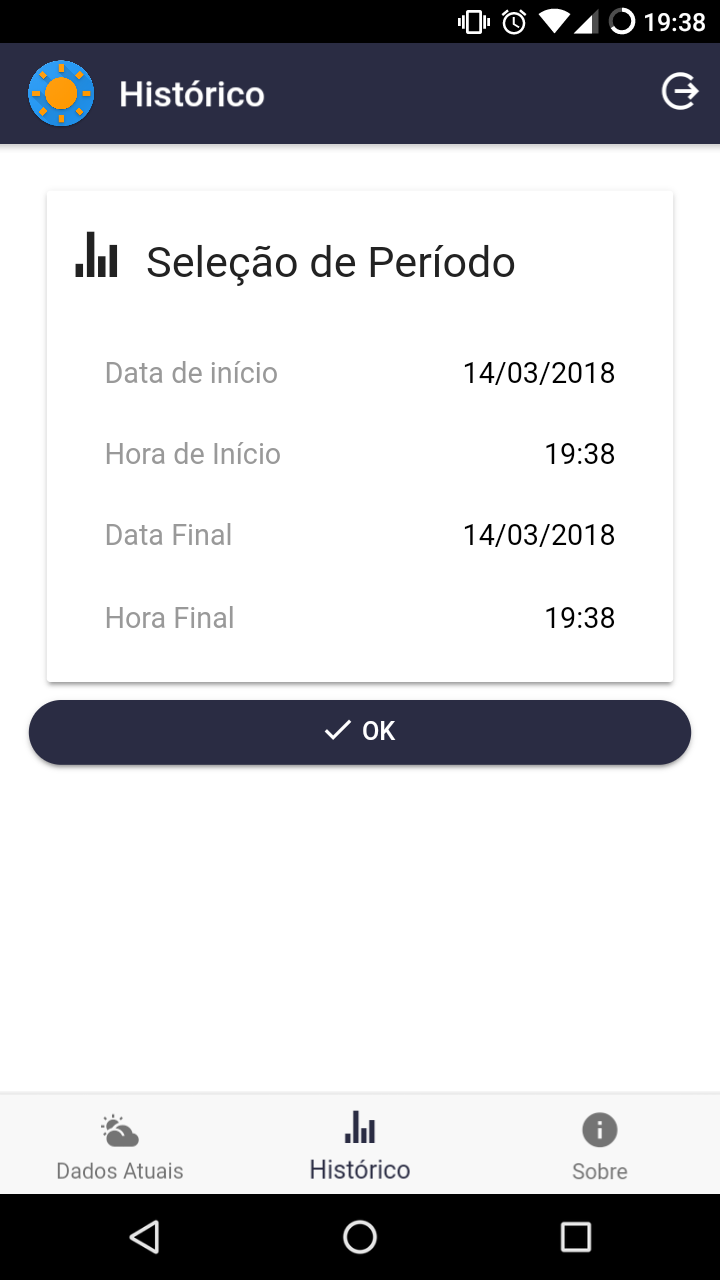
\includegraphics[scale=.15]{img/APP/periodo}}\qquad
    \subcaptionbox{\label{img:hist-rel}Exibir histórico}{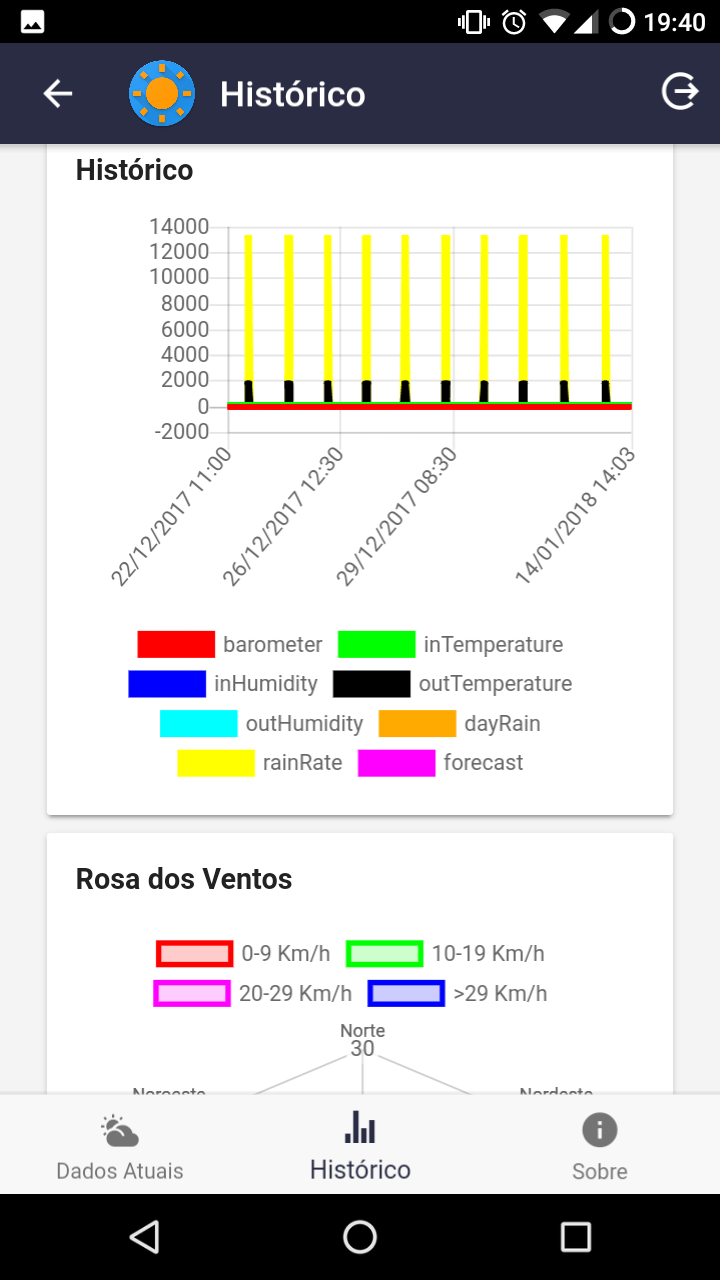
\includegraphics[scale=.15]{img/APP/historico}}\\
    \vspace{2.5em}
    \legend{\textbf{Fonte:} O Autor}
\label{fig:dag}
\end{figure}


Será sempre permitido ao usuário retornar para a tela anterior através do botão voltar, com exceção das telas de \textit{login} e cadastro, que só serão acessíveis se o usuário realizar \textit{logoff} ou reinstalar a aplicação. O fluxo de funcionamento da aplicação cliente é representado pelo diagrama de atividades da figura \ref{img:atividades1} na subseção \ref{subsec:diagAtiv}.

A figura \ref{img:login} mostra a tela utilizada no caso de uso de autenticação do usuário. A figura \ref{img:dados_atuais} mostra a tela de visualização dos dados atuais. As figuras, \ref{img:hist-time} e \ref{img:hist-rel} correspondem ao caso de uso de visualização de histórico.

\subsection{A API do sistema} \label{subsec:api}

Os URIs da API do sistema estão mostrados na tabela \ref{tab:api} abaixo. A tabela divide-se em três partes, a primeira representa as ações que podem ser executadas por um usuário não autenticado, a segunda evidencia as ações possíveis para um usuário que efetuou \textit{login} e a terceira expõe as ações internas do sistema.

%\definecolor{Gray}{gray}{0.85}
%\newpage

\begin{table}[!h]
\huge
\centering
\caption{\label{tab:api} API RESTful do sistema.}
\begin{adjustbox}{max width=\textwidth}
\begin{tabular}{@{} p{8.5cm} l l p{10cm} @{}}
\hline
\multicolumn{1}{c}{\textbf{Ator}}                             & \multicolumn{1}{c}{\textbf{Método}} & \multicolumn{1}{c}{\textbf{URI}}                 & \multicolumn{1}{c}{\textbf{Descrição}}                                                    \\ \hline
\multicolumn{1}{l|}{\multirow{2}{*}{Usuário não autenticado}} & POST                                & \multicolumn{1}{l|}{/auth/login}                 & Autentica o usuário utilizando os parâmetros passados no corpo da requisição;                                                                      \\ \cline{2-4} 
\multicolumn{1}{l|}{}                                         & POST                                & \multicolumn{1}{l|}{/auth/register}              & Cria um novo usuário com os parâmetros passados no corpo da requisição;                   \\ \hline
\multicolumn{1}{l|}{\multirow{2}{*}{Usuário autenticado}}     & GET                                 & \multicolumn{1}{l|}{/read/last}                  & Retorna o último documento da base de dados;                                              \\ \cline{2-4} 
\multicolumn{1}{l|}{}                                         & GET                                 & \multicolumn{1}{l|}{/read/:readMoment1/:readMoment2} & Retorna os dados contidos período especificado pelos parâmetros da requisição;                                           \\ \hline
\multicolumn{1}{l|}{Sistema}                                  & POST                                & \multicolumn{1}{l|}{/read}                       & Cria um novo documento no banco com os valores das variáveis passados no corpo da requisição; \\ \hline                          
\end{tabular}
\end{adjustbox}
\legend{\textbf{Fonte:} O Autor}
\end{table}


\subsection{Modelos de dados do sistema} \label{subsec:datamodel}

O banco de dados escolhido para a implementação do projeto é não-relacional baseado em documentos. Os documentos podem conter vários pares chave-valor, ou vários pares chave-vetor, ou até vários documentos encadeados. A estrutura do documento é flexível, o que permite alterações e inserções futuras de dados novos em uma base preexistente \cite{SITEMONGODB}. Um dos modelos de dados adotado para o projeto é mostrado na figura \ref{img:collection} abaixo, onde de um lado têm-se as chaves representando os dados fornecidos pela estação e do outro seus respectivos valores.

Os valores de cada chave adotada para o modelo de documentos são providos pelo \textit{datalogger} da estação. As chaves possuem o valor obtido diretamente dos sensores.


\newpage
\imagem{0.55}{collection}{Modelo de documento das leituras do sistema}{O Autor}


O outro modelo de dados do sistema é referente aos dados de usuário, como indicados na figura \ref{img:collection2}. Os valores desses dados são preenchidos no momento do cadastro do usuário. Neste momento o sistema criptografa a senha enviada, por meio do algortimo \textit{bcrypt}, e salva somente a senha criptografada no banco. 

\imagem{0.55}{collection2}{Modelo de documento dos usuários do sistema}{O Autor}